\documentclass[../notes.tex]{subfiles}
\begin{document}
\section{Day 2}
\subsection{The Fundamental Group}
    \begin{itemize}
        \item Idea: $\pi_1(X)=\faktor{\{\text{``loops'' in X}\}}{\sim}$, where $L_1 \equiv L_2$ if $L_1$ can be ``deformed'' inside $X$
            into $L_2$
        \item \underline{Ex:} Last time it was claimed that $\pi_1(\R^2\setminus \{(0,0)\})=\Z$.
        \item\underline{Paths and Homotopies}
        \item Let $X$ be a topological space.
    \end{itemize}
        \begin{definition}
            A \underline{path} in $X$ is a continuous map $f:I \rightarrow X$, where $I=[0,1]\subseteq \R$ (with the
            subspace topology from the Euclidean topology on $\R$.)\\
            If $f(0)=p$ and $f(1)=q$, we say $f$ is a path \underline{from $p$ to $q$}.
        \end{definition}
    \begin{itemize}
        \item \underline{Ex:}
            \begin{align*}
                X&=\R^2\\
                f: I &\rightarrow\R^2\\
                f(t)&=(1-2t,0)\\
            \end{align*}
            $f$ is a path in $\R^2$ from $(1,0)$ to $(-1,0)$.
        \item Another path in $\R^2$ from $(1,0)$ to $(-1,0)$ is,
            \begin{align*}
                g: I &\rightarrow \R^2\\
                g(t)&=(\cos(\pi t),\sin(\pi t))\\
            \end{align*}
        \item To make precise, ``Deforming'' one path into another:\\
            \begin{center}
                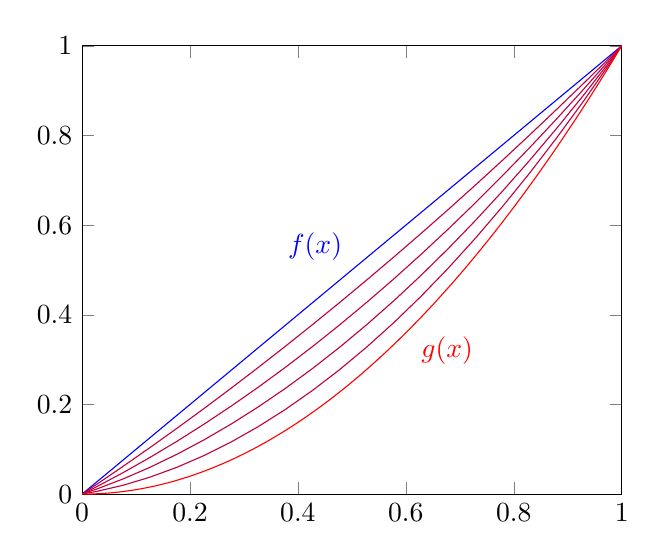
\begin{tikzpicture}
                    \begin{axis}[
                        xmin=0,xmax=1,
                        ymin=0,ymax=1
                        ]
                        \addplot [samples=200,color=blue, domain=0:1]{x}
                        node [color=blue,pos=.5,above left] {$f(x)$};
                        \addplot [samples=200,color=purple]{.8*x+.2*x^2};
                        \addplot [samples=200,color=purple]{.6*x+.4*x^2};
                        \addplot [samples=200,color=purple]{.4*x+.6*x^2};
                        \addplot [samples=200,color=purple]{.2*x+.8*x^2};
                        \addplot [samples=200,color=red, domain=0:1]{x^2}
                        node [color=red,pos=.5,below right] {$g(x)$};
                    \end{axis}
                \end{tikzpicture}
            \end{center}
    \end{itemize}
        \begin{definition}
            Let $f$ and $g$ be paths in $X$ from $p$ to $q$. A \underline{path homotopy} from $f$ to $g$ is a continuous function,
            \begin{align*}
                H: I\times I \rightarrow X\
            \end{align*}
            (note that elements of $I\times I$ resemble, $(s,t)$)
            Such that,
            \begin{align*}
                H(s,0)&=f(s),\ \forall s\\
                H(s,1)&=g(s),\ \forall s\\
                H(0,t)&=p,\ \forall s\\
                H(1,t)&=q,\ \forall s\\
            \end{align*}
        \end{definition}
    \begin{itemize}
        \item
            To make sense of this, define, $\forall t$,
            \begin{align*}
                h_t: I&\rightarrow X\\
                h_t(s)&=H(s,t)\\
            \end{align*}
            Then, $\forall t$,
            \begin{align*}
                h_t= \text{ path in $X$ from $p$ to $q$ }\\
            \end{align*}\\
            \begin{center}
                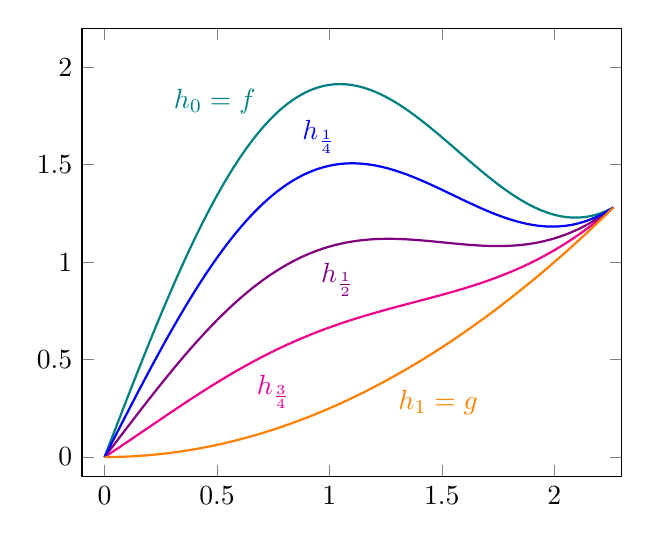
\begin{tikzpicture}
                    \begin{axis}[
                            xmin=-.1,xmax=2.3,
                            ymin=-.1,ymax=2.2
                        ]
                        \addplot [samples=200,color=teal,domain=0:2.263,thick]{
                            sin(deg(2*x))+x
                        }
                        node [above left, pos=.5,color=teal,thick]{$h_0=f$};
                        \addplot [samples=200,color=magenta,domain=0:2.263, thick]{
                            .25*(sin(deg(2*x))+x)+.75*((x^2)/4)
                        } node [below right, color=magenta,pos=.30] {$h_{\frac{3}{4}}$};
                        \addplot [samples=200,color=violet,domain=0:2.263, thick]{
                            .5*(sin(deg(2*x))+x)+.5*((x^2)/4)
                        } node [below right, ,pos=.5, thick] {$h_\frac{1}{2}$};
                        \addplot [samples=200,color=blue,domain=0:2.263, thick]{
                            .75*(sin(deg(2*x))+x)+.25*((x^2)/4)
                        } node [above left, color=blue,pos=.6] {$h_\frac{1}{4}$};
                        \addplot [samples=200,color=orange,domain=0:2.263, thick]{(x^2)/4}
                        node [below right, color=orange,pos=.5] {$h_1=g$};
                    \end{axis}
                \end{tikzpicture}
            \end{center}
            This is continuous because $H$ is continuous, and it goes from $p$ to $q$, because $h_t(0)=H(0,t)=p$ and $h_t(1)=H(1,t)=q$.
            $h_0(s)=f$ because $h_0(s)=H(s,0)=f(s),\ \forall s$\\
            and $h_1(s)=g$ because $h_1(s)=H(s,1)=g(s),\ \forall s$\\
    \end{itemize}
    \begin{definition} If $\exists$ a path homotopy from $f$ to $g$, we say $f$ and $g$ are \underline{path-homotopic}, and $f\cong g$\\
        \underline{Ex:} $X=\R^2$, Let,
        \begin{align*}
            f(s)=(\cos(\pi s), \sin(\pi s))\\
            f(s)=(\cos(\pi s), 2\sin(\pi s))\\
        \end{align*}
        Both are paths in $\R^2$ from $(1,0)$ to $(-1,0)$.\\
        Then,
        \begin{align*}
            H: I\times I &\rightarrow \R^2\\
            H(s,t)&=(\cos(\pi s), (t+1)*\sin(\pi s))\\
        \end{align*}
        $H$ is a path homotopy from $f$ to $g$, because,
        \begin{align*}
            H(s,0)&=(\cos(\pi s), \sin(\pi s))=f(s)\\
            H(s,1)&=(\cos(\pi s), 2\sin(\pi s))=g(s)\\
            H(0,t)&=(\cos(0), (t+1)\sin(0))=(1,0)\forall t\\
            H(1,t)&=(\cos(\pi), (t+1)\sin(\pi))=(-1,0)\forall t\\
        \end{align*}
    \end{definition}
    \begin{itemize}
        \item \underline{Question:} Find a path homotopy from $\R^2$ from $f(s)=(s,s)$, and $g(s)=(s,s^2)$\\
            Answer(June): $H(s,t)=(s,s^{t+1})$\\
            (see the notebook, there's a solution there. Keep in mind that you want to try to find $p$ and $q$ first, before you do anything else)\\
            Answer(Dr. Clader): General Trick In $\R^2$ let $f$ and $g$ be any two paths from $p$ to $q$, then the
            \underline{straight line homotopy} is as follows,
            \begin{align*}
                H: &I \times I \rightarrow \R^2\\
                H(s,t)&=(1-t)*f(s)+t*g(s)\\
            \end{align*}
            Note that this resembles the stuff you've seen in optimization and advanced linear algebra. This is a pretty powerful tool,
            remember and fear it.
        \item \underline{Ex:} In the question above, $H(s, t)=(s, (1-t)s+ts^2)$
    \end{itemize}
\end{document}
